\chapter{Requirement Analysis and System Specifications}
\section{Feasibility Study}
Depending on the results of the initial investigation, the survey is expanded to a
more detailed feasibility study. Feasibility study is a test of system proposal ac-
cording to its work ability, impact on the organization, ability to meet user needs,
and effective use of resources. The objective for this phase is not to solve the
problem but to acquire a sense of scope. During the study, the problem definition
is crystallized and aspects of the problem to be included in the system are deter-
mined.\\ \\
Mobile Application Development Systems are capital investments because resources
are being spent currently in order to achieve benefits to be received over a pe-
riod of time following completion. There should be a careful assessment of each
project before it is begun in terms of economic justification, technical feasibility,
operational impact and adherence to the master development plan.
We started the project by listing the possible queries that the user might want
to be satisfied. And on these lines we guided the project further.\\ \\
The three main points, kept in mind at the time of project, are :
\begin{itemize}
\item Possible (To build it with the given technology and resources)
\item Affordable (given the time and cost constraints of the organization)
\item Acceptable (for use by the eventual users of the system
\end{itemize}

The three major areas to be considered while determining the feasibility of a
project are :
\begin{enumerate}
\item \textbf{\emph{Technical Feasibility:}} The technical issue usually raised during the feasi-
bility stage of the investigation includes the following :
\begin{itemize}
\item Does the necessary technology exist to do what is suggested?
\item Do the proposed equipments have the technical capacity to hold the
data required to use the new system?
\item Will the proposed system provide adequate response to inquiries, re-
gardless of the number or location of users?
\item Can the system be upgraded if developed?
\item Are there technical guarantees of accuracy, reliability, ease of access
and data security?
\end{itemize}

Earlier no system existed to cater to the needs of ’Secure Infrastructure Im-
plementation System. The current system developed is technically feasible.
It is a web based user interface. Thus it provides an easy access to the
users. The databases purpose is to create, establish and maintain a work-
flow among various entities in order to facilitate all concerned users in their
various capacities or roles. Permission to the users would be granted based
on the roles specified.
Therefore, it provides the technical guarantee of accuracy, reliability and
security. The software and hardware requirements for the development of
this project are not many and are already available as free as open source.
The work for the project is done with the current equipment and existing
software technology. Necessary bandwidth exists for providing a fast feed-
back to the users irrespective of the number of users using the system.

\item \textbf{\emph{Operational Feasibility:}} Under this category of service we conduct a study to analysis and determine whether your need can be fulfilled by using a proposed solution. The result of our operational feasibility Study will clearly outline that the solution proposed for your business is operationally workable and conveniently solves your problems under consideration after the proposal is implemented. We would precisely describe how the system will interact with the systems and persons around. Our feasibility report would provide results of interest to all stakeholders. It will do as per the needs of the business requirements.

\item \textbf{\emph{Timeline Feasibility:}} It is important to understand that a need must be fulfilled when it has to be. Some otherwise feasible and highly desirable projects can become non-feasible due to very restrictive timeline constraints. This fact makes it imperative that milestones are clearly linked to the timeline and projects are well conceived with safe unforeseen margins. We make sure that we strictly follow what has been stated above.

\end{enumerate}

\pagebreak

\section{Software Requirement Specification Document}

\subsection{Data Requirements}
Data requirement is meant to be the data that will be used in our application. Data required in this project is all notices, that need to be conveyed to the user. This application also require the username and passwords of persons in order to register them and sending notification about updates. So two main requirements are:
\begin{itemize}
\item {Notice Details}
\item {User Details}
\end{itemize}

\subsection{Functional Requirements}
In order to make this application functional, we require the following:
\begin{itemize}
\item \textbf{\emph{Download mobile application:}}\\
A user should be able to download the mobile an
application through either an application store or
similar service on the mobile phone. The application should be free to download.
\item \textbf{\emph{User registration:}}\\
Given that a user has downloaded the mobile application, then the user should be able to register
through the mobile application. The user must provide user-name, password and e-mail address. The user 
can choose to provide a regularly used phone number.

\item \textbf{\emph{User Login:}}\\
Given that a user has registered, then the user should be able to log in to the mobile application.
The log-in information will be stored on the phone and in the future the user should be logged in automatically. 

\item \textbf{\emph{Reset Password:}}\\
Given that a user has registered, then the user should be able to retrieve his/her password by e-mail. 

\item \textbf{\emph{DashBoard:}}\\
Given that a user is logged in to the mobile application, then the first page that is shown should be
the dashboard page. The user should be able to see all the college notices.

\item \textbf{\emph{Search Notice:}}\\
The user should be able to search for a notice by its title. For example, if a user types fee, all the notices having fee in their content get displayed.

\item \textbf{\emph{Selecting a Notice:}}\\
 A user should be able to select any notice from list view. The click on particular notice will take him to notice details
 of that particular notice.

\item \textbf{\emph{Navigating back to Notices List:}}\\
The user should be able to navigate back to notices list from the notice details section. This is required to give a 
good user experience.

\item \textbf{\emph{Deleting Notices:}}\\
The user should have the option to delete the unnecessary notices from his phone, by ticking them one by one and then deleting them in one go. This way, user can save this phone memory from unrequired notices.

\item \textbf{\emph{Posting Notices:}}\\
The admin of this application should be able to post the notices. He should be able to add a picture within notices. That picture
can be taken either from gallery or by using the camera of the mobile phone.

\item \textbf{\emph{Notification Alert:}}\\
All the registered users should be able to have a ping or notification on their mobile phone whenever a new notice is posted.

\end{itemize}

\subsection{Performance Requirements}
The requirements in this section provide a detailed specification of the user interaction with the software and measurements placed on the system performance.
\begin{itemize}
\item \textbf{\emph{Prominent search feature:}}\\
The search feature should be prominent and easy to find for the user.

\item \textbf{\emph{Usage of the Notice Information:}}\\
The notice link should be prominent and it should be evident that it is a usable link.
Selecting the notice link should only take one click.

\item \textbf{\emph{Response Time:}}\\
The reponse time should not be more than 5 seconds if user have a proper internet connection. 

\item \textbf{\emph{Fault Tolerance:}}\\
The fault tolerance of the system should be very good. If the system loses the connection to the Internet or the system gets some 
strange input, the user should be informed.

\end{itemize}

\subsection{System Dependability}
Following are the requirements that an application require from the device/mobile on which it is installed.
\begin{itemize}
\item \textbf{\emph{Internet Permission:}}\\
Application develeped, require full internet permissions of mobile so that it can fetch notices from the server.
At the same time, it should be able to receive buzz or notification tone whenever new notice is posted by admin.

\item \textbf{\emph{External SD Card Writable Permissions:}}\\
This application would be requiring read write access to SD card. It is required in order to download the notices attachment and save
in SD card of mobile phone.

\item \textbf{\emph{System Tools:}}\\
This application require various system tools to be used. For example, it requires Camera of mobile in order to click the image and
post in into notice. It also require system tool, that prevents it from sleeping.

\item \textbf{\emph{Hardware Control:}}\\
It uses vibrator of mobile phone whenever any notification arrives.

\item \textbf{\emph{Account Info:}}\\
It also fetches your google account information in order to get the user registered with Google Cloud Messaging.
\end{itemize}

\subsection{Maintainability Requirements}
Following are the maintainability requirement of e-Notice mobile application:
\begin{itemize}

\item \textbf{\emph{Application extendibility:}}\\
The application should be easy to extend. The code should be written in a way that it favors
implementation of new functions. It is requires in order for future functions to be implemented easily to the application.

\item \textbf{\emph{Application testability:}}\\
Test environments should be built for the application to allow testing of the applications different
functions.

\end{itemize}

\subsection{Security Requirements}
\begin{itemize}
\item \textbf{\emph{Communication Security:}}\\
There shoulb be security of the communication between the system and server.The messages should be
 encrypted for log-in communications, so others cannot get user-name and password from those messages.
Every exchanged of information between client and server should be encrypted so that no one can track it.
\item \textbf{\emph{Admin Login Account Security:}}\\
If an admin tries to log in to the web portal with a non-existing account then the admin should
not be logged in. The admin should be notified about log-in failure.
\item \textbf{\emph{Admin Account Security:}}\\
There should be security of admin accounts. An admin and IP address should not be able to log-in to the web portal for a certain time period
after three times of failed log-in attempts.

\item \textbf{\emph{User Create Account Security:}}\\
The security of creating account for users of the system should be maintained. If a user wants to
 create an account and the desired user name is occupied, the user should be asked to choose a different user name.
\end{itemize}
\subsection{Look and Feel Requirements}

Regarding look and feel, our client is straight forword. They believe in simplicity. So these are their requirements:
\begin{itemize}
\item \textbf{\emph{Simple and Light:}}\\
The user interface should be simple and lightly colored. It should give relaxing effect on looking at its GUI. No bright
colors should be used while designing the UI of this application.

\item \textbf{\emph{Easy to Use}}\\
The application should be easy to use. If any user is doing something wrong, he/she should be informed correctly, what is going
wrong behind the scene. There should be proper instructions for the user to use this application.

\item \textbf{\emph{Soft Sound Notification:}}\\
The sound for notification should be very soft. It should not distrub the pers with a loud note.
Everything should be sober in this application.
\end{itemize}

%%%%%%%%%%%%%%%%%%%%%%%%%%%%%%%%%%%%%%%%%%%%%%%%%%%%%%%%%%%%%%%%%%%%%%%%%%%%%%%%%%%%%%%%%%%%%%%%%%%%%%%%%%%%%%%%%%%%%%%%%%%%%%%%
\pagebreak
\section{Validations}
Any application is useless without validation. There should be a way to validate the user input first before sending the user request to the server. Following are the validations implemented in proposed system:
\begin{itemize}
\item \textbf{\emph{User Password Validation:}}\\
The application should check the user and password fields before sending any request to the server. It should check whether the fields are
filled or not. if fields are not filled up, user should be instructed to fill up the fields before moving further. in this way, there will
be less traffic on the server.

\item \textbf{\emph{Validations During Registration:}}\\
There are a lot of validations that needs to be implemented in the application. They are as follow:
\begin{enumerate}

\item \textbf{\emph{First and Last Name of User:}}\\
The first and last name of user should be not null. Also first letter of first and last name should be in uppercase.

\item \textbf{\emph{Username:}}\\
The username can contain only alphabets, digits, underscore and hyphen. It should be atleast 3 characters long and maximum of 15 characters.

\item \textbf{\emph{Password:}}\\
The password must contains one digit from 0-9, one lowercase character,one uppercase character, one special symbols in the list "\@\#\$\%" and length of password must be at least 6 characters and maximum of 20.

\item \textbf{\emph{Email:}}\\
The application must validate and email address entered by the user before sending request to the server.

\item \textbf{\emph{Mobile Number:}}\\
The mobile number should be of only ten digits. No more, no less than that.
\end{enumerate}

\item \textbf{\emph{Validating During Posting Notices:}}\\
The application should validate the notice posting fields before posting any notice. It should check whether title and description fields are filled or not. if not, it should tell the user to fill up the required fields while posting the notice.

\item \textbf{\emph{Reset Password Validation:}}\\
The application should check that user has entered the username or email in the given filed before pressing the reset password button.

\end{itemize}

%%%%%%%%%%%%%%%%%%%%%%%%%%%%%%%%%%%%%%%%%%%%%%%%%%%%%%%%%%%%%%%%%%%%%%%%%%%%%%%%%%%%%%%%%%%%%%%%%%%%%%%%%%%%%%%%%%%%%%%%%%%%%%%%%%%%
\pagebreak
\section{Expected Hurdles}
The main hurdles that can come in the notice are as follow:
\begin{enumerate}
\item \textbf{\emph{GCM Notification:}}\\
Its possible that there may be a problem with receiving GCM notifications. When to receive a broadcast signal and when to start the service.
If service is not started at the proper time, there may be the case, user will not be able to receive any notification from the server.

\item \textbf{\emph{Device Database:}}\\
Its very much difficut to see entries going inside the device database. You have to check through coding. You can't access the applications database easily. So its bit hard to debug the database errors.

\item \textbf{\emph{Device SD Card:}}\\
The application will be requiring access to the SD card of the user mobile. It may be possible that SD Card is full or missing SD Card. So the user will not be able to receive the respective attachment of notices.

\item \textbf{\emph{Google Play Services:}}\\
Registering to the GCM Server requires to have Google Play services on device installed. Otherwise user will not be able to register 
to GCM server nor will be able to receive any message.
\end{enumerate}

%%%%%%%%%%%%%%%%%%%%%%%
\pagebreak
\section{SDLC Model Used}
This section describes the project as per the various stages of the Software Development life
cycle. The model of software development life cycle used in this project is the waterfall method.
The Waterfall Method is comprised of a series of very definite phases, each one run intended to
be started sequentially only after the last has been completed, with one or more tangible
deliverables produced at the end of each phase of the waterfall method of SDLC. Essentially, it
starts with a heavy, documented, requirements-planning phase that outlines all the requirements
for the project, followed by sequential phases of design, coding, test-casing, optional
documentation, verification (alpha-testing), validation (beta-testing), and finally
deployment/release.\\


\begin{figure}[H]
\centering 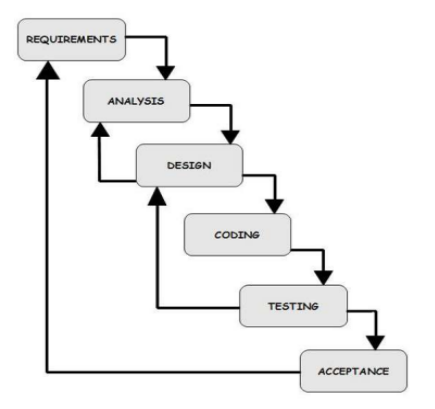
\includegraphics[scale=0.7]{image/sdlc.png}
\caption{Login Page}
\end{figure}
\begin{enumerate}
\item \textbf{\emph{Requirement Analysis:}}\\
Existing system is time consuming and it makes difficult to convey huge amount of users about
any event, class or seminar almost instantly. Also there is always a big crowd in front of
noticeboard. So it was hectic to read any useful instruction and information. Thus all the
problems of the existing system are summarized and proposing a new system that works as an
online application. It is a value added solution to the problem. It resolves all the problems stated
above. It will provide simple interface to the user to operate on and convey the intended users
about events almost instantly, anytime and anywhere.
\item \textbf{\emph{Design:}}\\
It includes translation of the requirements specified in the SRS into a logical structure that can be implemented in a programming language. The output of the design phase is a design document that acts as an input for all the subsequent SDLC phases. The design of this app is simple and user friendly containing six main activities, namely:
\begin{enumerate}
\item Register 
\item Login
\item Dashboard
\item Details of Notices
\item Admin Panel 
\item Reset Password
\end{enumerate}

\item \textbf{\emph{Coding/Implementation:}}\\
It includes translation of the requirements specified in the SRS into a logical structure that can be implemented in a programming language. The output of the design phase is a design document that acts as an input for all the subsequent SDLC phases. The project is implemented using the Android virtual devise (AVD). This emulator helped to implement the project in a real-like environment and sketch out the details of how it will work on a real hardware. Each activity is linked with another and interconnectivity is transparent and smooth.

\item \textbf{\emph{Testing:}}\\
It includes detection of errors in the application. The testing process starts with a test plan that recognizes test-related activities, such as test case generation, testing criteria, and resource allocation for testing. The code is tested and mapped against the design document created in the design phase. The output of the testing phase is a test report containing errors that occurred while testing the application. Testing of the project has not been done on  real hardware and also on the emulator or software environment. Testing has been done for each of the individual activities of the project.

\item \textbf{\emph{Maintenance:}}\\
It includes implementation of changes that software might undergo over a period of time, or implementation of new requirements after the software is deployed at the customer location. The maintenance phase also includes handling the residual errors that may exist in the software even after the testing phase. The project maintenance is low cost and efficient as user will get this application at free of cost and also this application is shared over network, therefore maintenance is little bit difficult. 

\end{enumerate}
